\chapter{Introduction}
The canton of Grisons is located in south-east Switzerland and is officially a trilingual canton, with German as the main language, followed by Romansh and Italian. This grammar is about a Romansh variety.

Romansh has six different written standard varieties. Five of them developed naturally out of the contact between Latin and not clearly identified substrate languages: Sursilvan, Sutsilvan, Surmiran, Putér, and Vallader. In the Protestant parts of Romansh Grisons, the varieties started to be written in the 16th century, mostly for religious purposes (Putér, Vallader, and Sutsilvan), and in the Catholic parts a century later (Sursilvan and Surmiran). 

Rumantsch Grischun is an artificial language created in 1982 by Heinrich Schmid on behalf of the Lia Rumantscha, the umbrella association of all the Romansh language organisations. Heinrich Schmid was a Romance philologist from the University of Zurich (Switzerland). Rumantsch Grischun is used above all for official purposes by the canton of Grisons and the Swiss Confederation.

Sursilvan, Sutsilvan, Putér and Vallader are used as the language of instruction in their respective areas; Rumantsch Grischun is only used in the Surmiran area. However, after the vote on July 24, 2020, Surmiran will be reintroduced as the language of instruction up to the fourth grade of primary school in 2021. 

Tuatschin is a Sursilvan dialect spoken in the uppermost part of the Sursilvan area by approximately 800 to 1000 people. It is the Sursilvan dialect that differs the most from the Sursilvan standard variety. These differences, however, do not concern the most salient typological features of Sursilvan like the predicative \textit{-s} of masculine singular adjectives and participles (see §3.3.1 and §4.1.2.1), nouns and adjectives with stem alternations as \textit{iart} (\textsc{m.sg}) vs \textit{òrts} \textsc{(m.pl}) `garden(s)', and \textit{matgiart} (\textsc{m.sg} attributive) vs \textit{macòrts} \textsc{(m.sg} predicative as well as \textsc{m.pl}, both attributive and predicative) `ugly', or the conservation of the Latin diphthong \textsc{au} like in \textit{aur} `gold'.

Some differences between Tuatschin and Standard Sursilvan concern palatalisation phenomena, the treatment of monophthongs and diphthongs, some pronominal and verbal forms, the form of the negator, and the form of the dative marker. \tabref{difstand} lists some of these differences.

\begin{table}
	\caption{Differences between Tuatschin and Standard Sursilvan}
	\label{difstand}
	\begin{tabular}{lllll}
		\lsptoprule
		& Tuatschin &  Sursilvan & English\\
		\midrule
	palatalisation of ˈ\textsc{ka}  & \textit{marˈʨaw} & \textit{marˈkaw} & `city'\\
	& \textit{ˈʨɛzɐ} & \textit{ˈkazɐ} & `house'\\
	Surs. \textit{ɔ} before \textit{n} & \textit{aˈvawn} & \textit{aˈvɔn} & `before'\\
	\textsc{1sg} pronoun & \textit{ju} & \textit{jɛw} & `I'\\
	see & \textit{ju ˈvɛʦɐ} & \textit{jɛw ˈvɛzɐl} & `I see'\\
	negator	& \textit{ˈbeʨɐ} &  \textit{ˈbukɐ} & `not'\\
	dative marker & \textit{da} &  \textit{a}\\
				\lspbottomrule
	\end{tabular}
\end{table}

\figref{fig:surs}\footnote{\tiny
	\url{https://commons.wikimedia.org/w/index.php?curid=46241682}
	CC-By-SA 4.0
	\url{https://commons.wikimedia.org/wiki/User:Terfili}
} shows the distribution of the three languages of Grisons with its dialects. The label `Tuatschin' on the map also comprises the Medelin dialect, spoken to the east of the Tuatschin area.\footnote{There is a mistake in the legend of the map: It should be \textit{Putér} instead of \textit{Putèr}.}

\begin{figure}
	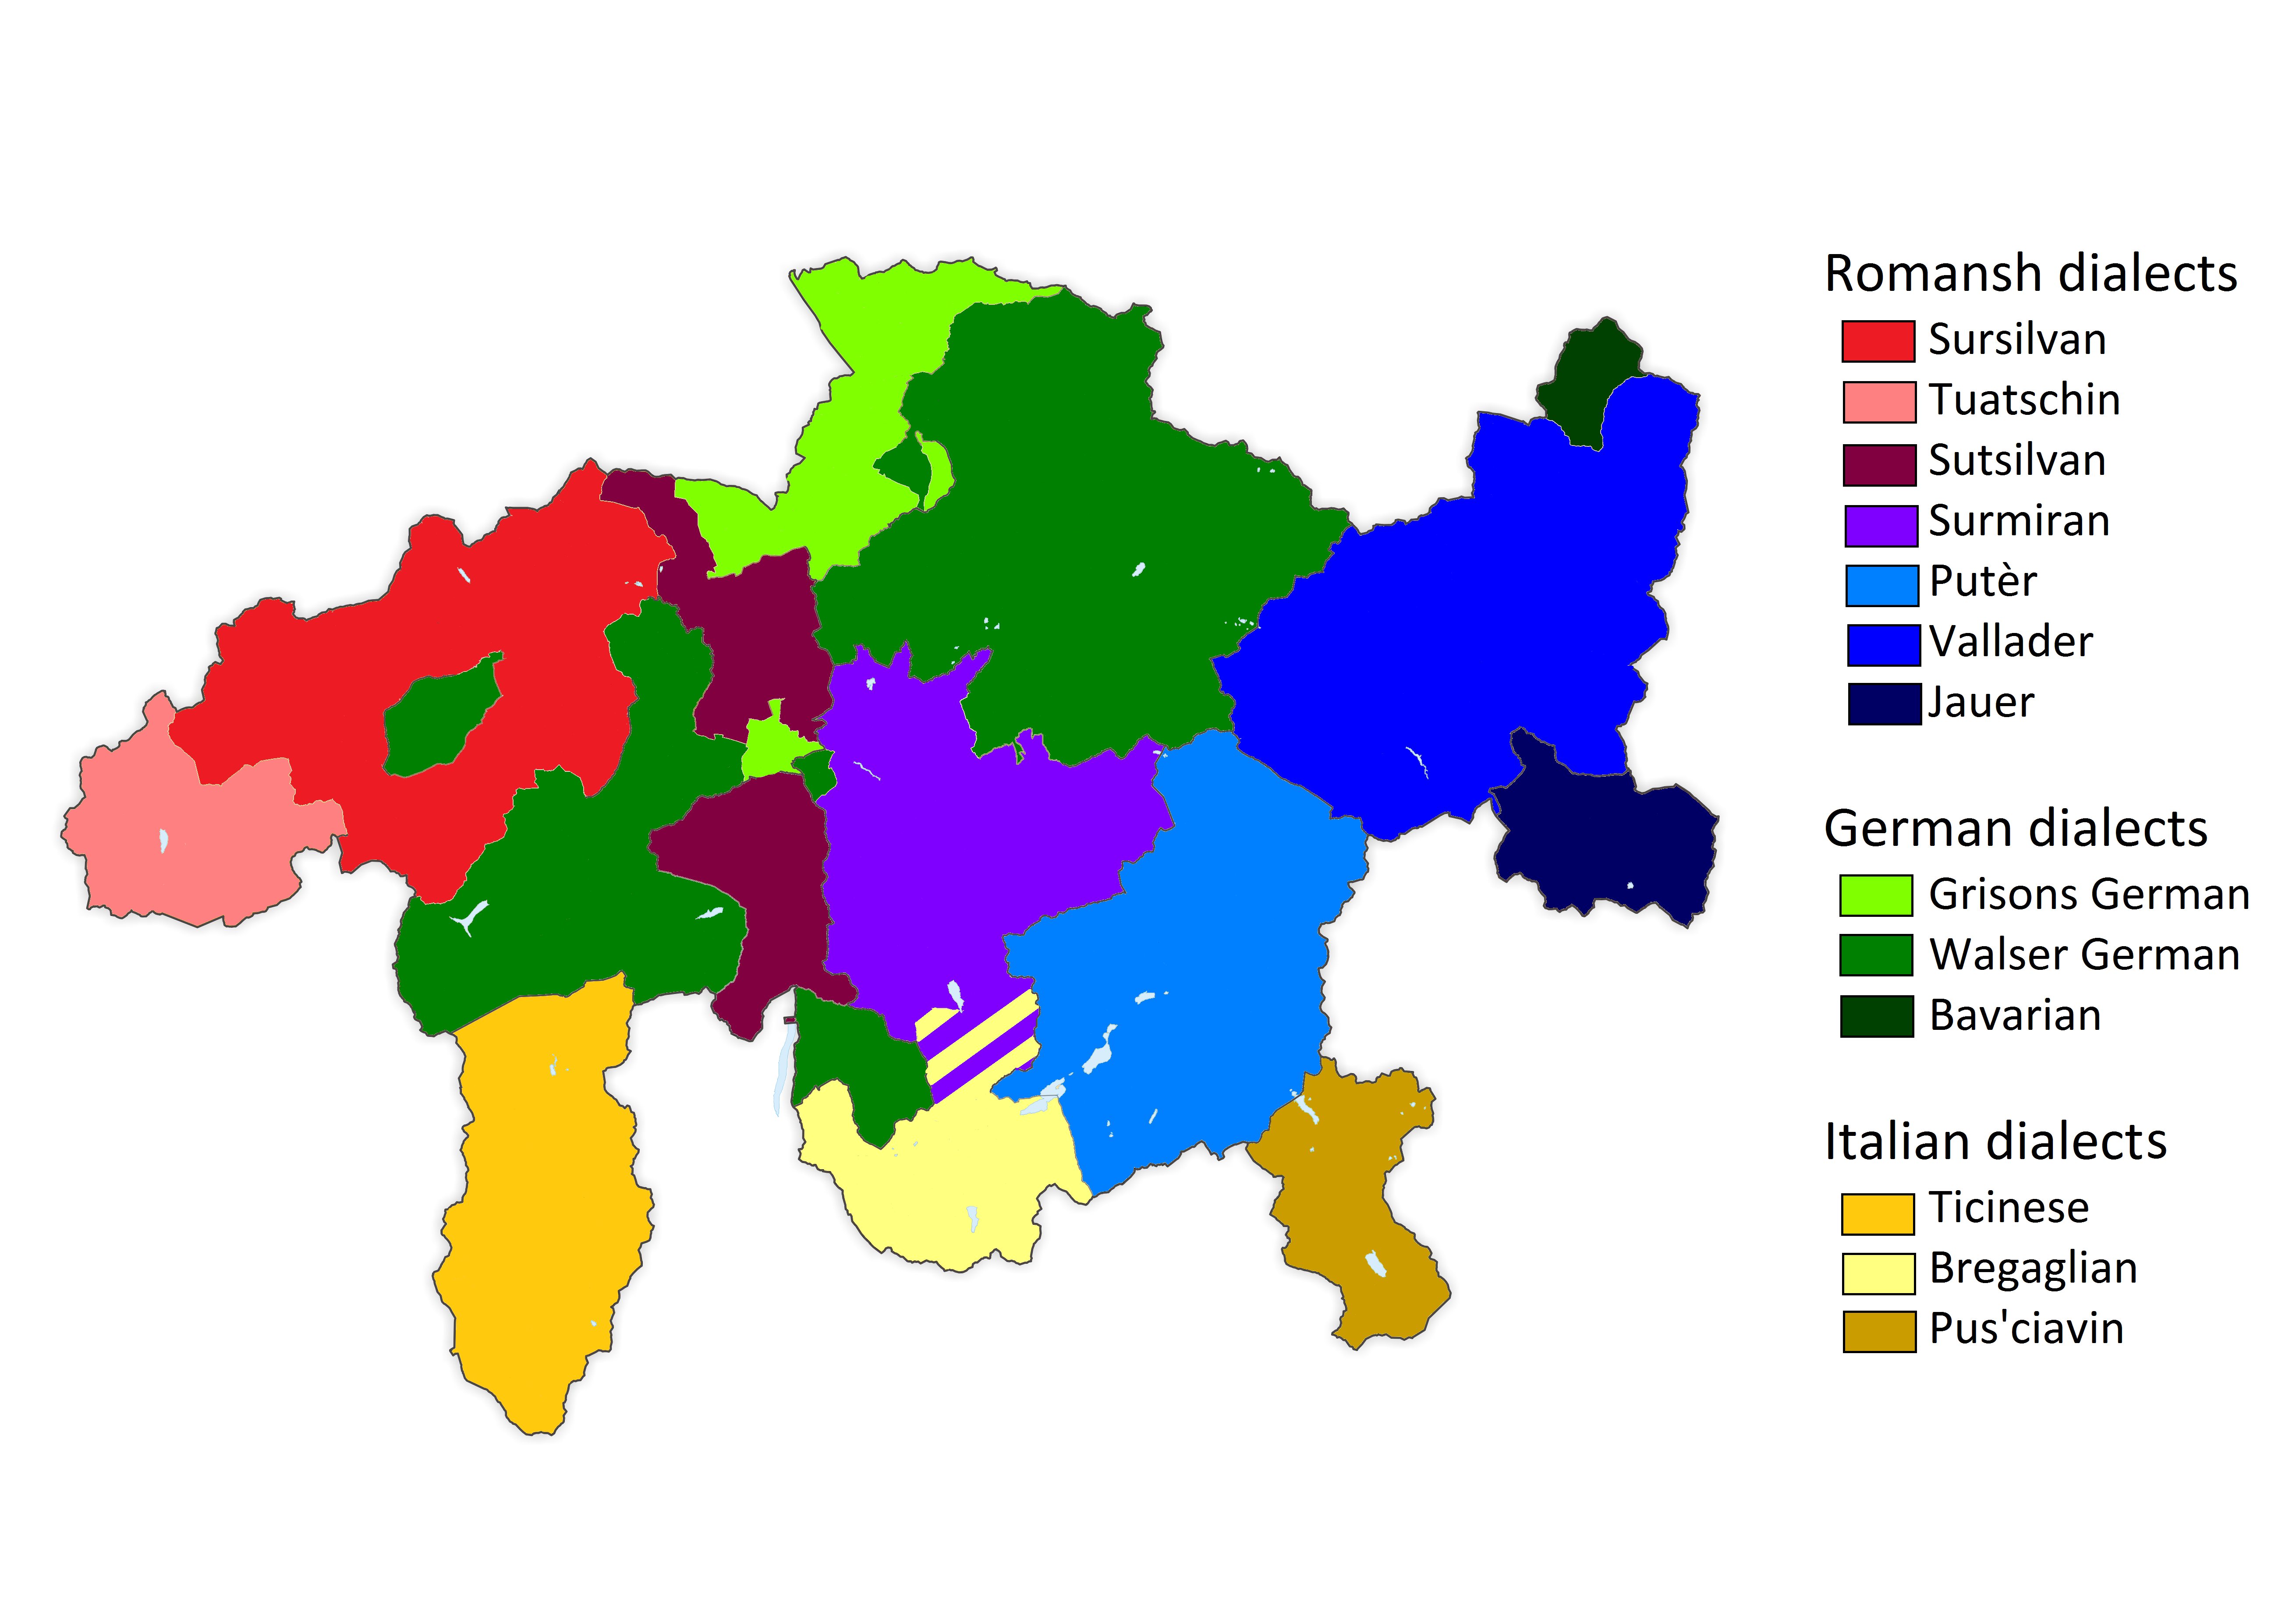
\includegraphics[height=.5\textheight]{figures/Languages Grisons.png}
	\caption{Languages and dialects of the Canton of Grisons}
	\label{fig:surs}
\end{figure}


\section{Previous works}
The most important linguistic study on Tuatschin is  \citet{Caduff1952}, \textit{Essai sur la phonétique du parler rhétoroman de la Vallée de Tavetsch}, which is about the diachronic phonetic development from Latin to Tuatschin. Some information about Tuatschin can also be found in \citet{VicHendry2010}, \textit{Tujetsch, ses vallers e lur tschontscha}. \citet{Maurer2017} analyses the marking of the indirect object from a diachronic perspective. 

There are some works containing Tuatschin texts and sentences; these will be mentioned in the next section.

\section{Corpus}
The corpus consists of oral and written sources. The oral corpus consists of two parts. The first part contains recorded narrations that were collected by myself on several field trips between 2016 and 2021 with seven female and ten male native speakers of Tuatschin; it consists of approximately 95 minutes of recorded stories told by male and female consultants between 30 and 82 years of age at the time of recording; they are published in chapter 8. The second part consists of elicited forms and sentences.

Since I have a working knowledge of Standard Sursilvan, all interviews were conducted in Romansh.

The most important written source of Tuatschin texts is \citet{Büchli1966}, \textit{Mythologische Landeskunde von Graubünden. 2. Teil: Das Gebiet des Rheins vom Badus bis zum Calanda}, which contains about 60, mostly short, traditional legends from the Tujetsch valley (specifying the village the story tellers were from) which were transcribed by the author himself. Büchli's consultants were born between 1858 and 1922.

The oldest texts I had access to was \textit{Il ratun tschiec} `The blind rat', which was published in 1889, and a transcribed text from the Schorta collection recorded in 1926 and published in \citet{Valär2013a} and \citet{Valär2013b}. Some sentences and dialogues can be found in the \textit{Dicziunari rumantsch grischun}, in \citet{Gartner1910}, \citet{Gadola1935}, Francestg \citet{Berther1998}, and in Baseli \citet{Berther2007}. 

The examples taken from the written sources were all adapted to the spelling system used in this book, with one exception, namely those written in IPA: \citet{Gartner1910}, as well as \citet{Valär2013a} and \citet{Valär2013b}.
  
The names of the consultants who participated in the project have been anonymised; their utterances will be labelled with a reference to their gender (f, m), and the place where they grew up. The female native speakers of Tuatschin consulted are listed in \tabref{tab:consultantsI} and \tabref{tab:consultantsII}, whereas the male native speakers are listed in \tabref{tab:consultantsIII} to \tabref{tab:consultantsV}. These lists contain their year of birth, the place where they grew up, and the mother tongue of their parents.

\begin{table}
	\caption{List of consultants I}
	\label{tab:consultantsI}
	\begin{tabular}{lllll}
		\lsptoprule
		& f1 & f2 & f3 & f4\\
		\midrule
		born & 1923 & 1937 & 1942 & 1947\\
		grew up in & Cavòrgja & Sèlva & Sadrún & Ruèras \\
		L1 mother & Tuatschín & Tuatschín & Tuatschín & Tuatschín \\
		L1 father & Tuatschín & Tuatschín & Tuatschín & Tuatschín \\
		\lspbottomrule
	\end{tabular}
\end{table}

\begin{table}
	\caption{List of consultants II}
	\label{tab:consultantsII}
	\begin{tabular}{llll}
		\lsptoprule
		& f5 & f6 & f7 \\
		\midrule
		born &  1961 & 1971 & 1972 \\
		grew up in &  Surajn &  Camischùlas &  Ruèras  \\
		L1 mother & Tuatschín & Tuatschín & Tuatschín\\
		L1 father & Sursilván & Tuatschín & Tuatschín\\
		\lspbottomrule
	\end{tabular}
\end{table}

\begin{table}
	\caption{List of consultants III}
	\label{tab:consultantsIII}
	\begin{tabular}{lllll}
		\lsptoprule
		& m1 & m2 & m3 & m4\\
		\midrule
		born & 1935 & 1934 & 1943 & 1949 \\
		grew up in & Ruèras & Zarcúns & Ruèras & Sadrún\\
		L1 mother & Tuatschín & Tuatschín & Tuatschín & Tuatschín\\
		L1 father & Tuatschín & Tuatschín & Tuatschín & Tuatschín\\
		\lspbottomrule
	\end{tabular}
\end{table}

\begin{table}
	\caption{List of consultants IV}
	\label{tab:consultantsIV}
	\begin{tabular}{lllll}
		\lsptoprule
		& m5 & m6 & m7 & m8\\
		\midrule
		born & 1952 & 1951 & 1953 & 1977\\
		grew up in & Sadrún & Sadrún & Cavòrgja & Sadrún\\
		L1 mother & Tuatschín & Tuatschín & Tuatschín & Tuatschín \\
		L1 father & Tuatschín & Tuatschín  & Tuatschín & Tuatschín\\
		\lspbottomrule
	\end{tabular}
\end{table}

\begin{table}
	\caption{List of consultants V}
	\label{tab:consultantsV}
	\begin{tabular}{lllll}
		\lsptoprule
		& m9 & m10\\
		\midrule
		born   & 1986 & 1943\\
		grew up in   &  Sadrún & Ruèras \\
		L1 mother & Tuatschín & Tuatschín\\
		L1 father  & Tuatschín & Tuatschín\\
		\lspbottomrule
		\end{tabular}
\end{table}

All consultants speak Tuatschin, Standard Sursilvan, Standard and Swiss German, and they are used to write in Standard Sursilvan and in Standard German. The young generation also uses Tuatschin in SMS and other social media.

Some decades ago, the people from Tujetsch would not use their own dialect with people from outside the Tujetsch valley, and still today some people are reluctant to speak Tuatschin with anybody who speaks Standard Sursilvan or another Sursilvan dialect. One of my consultants puts it this way:

\ea

\gll I drùva schòn in téc da saprèndar anzjaman da raṣdá da Tujétsch cun autars.\\
\textsc{expl} need.\textsc{prs.3sg} indeed \textsc{indef.m.sg} bit \textsc{attr} \textsc{refl}.take.\textsc{inf} together \textsc{comp} talk.\textsc{inf} of \textsc{pn} with other.\textsc{m.pl}\\
\glt `It needs indeed some [effort] to concentrate in order to speak Tuatschin with others.' (Zarcúns, m2)
\z

This explains in part why my consultants sometimes use Sursilvan forms when speaking with me.

\section{Dialectal differences}
There are two main Tuatschin dialects: the dialect of the upper part of the Tujetsch valley (\figref{fig:uppervalley}), which comprises the villages of Selva and Tschamut\footnote{According to \DRG{7}{636}, the inhabitants of Selva and Tschamut are called \textit{quèls dadajns gl uaut} `those above the forest'.}, and the dialect of the lower part of the valley (\figref{fig:lowervalley}), from Rueras to Bugnei. These two dialectal areas are divided by a forest called the forest of Sontga Brida \citep[3]{Caduff1952}. 

\begin{figure}
	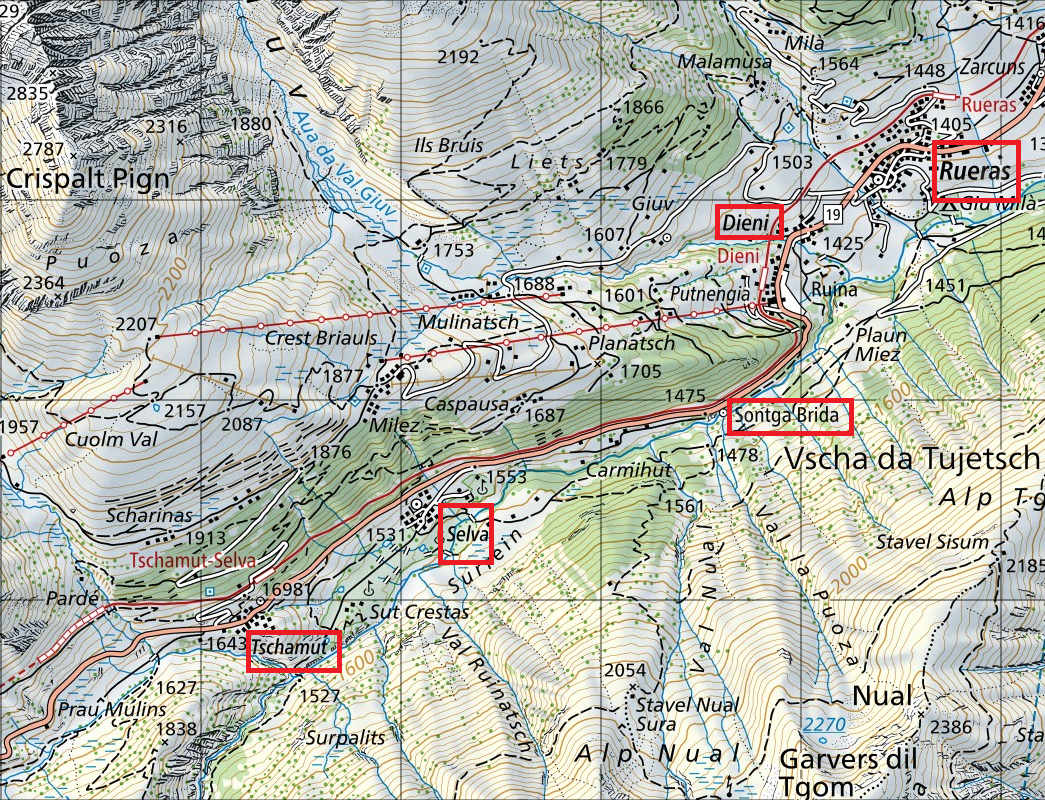
\includegraphics[height=.5\textheight]{figures/Upper Valley.png}
% 	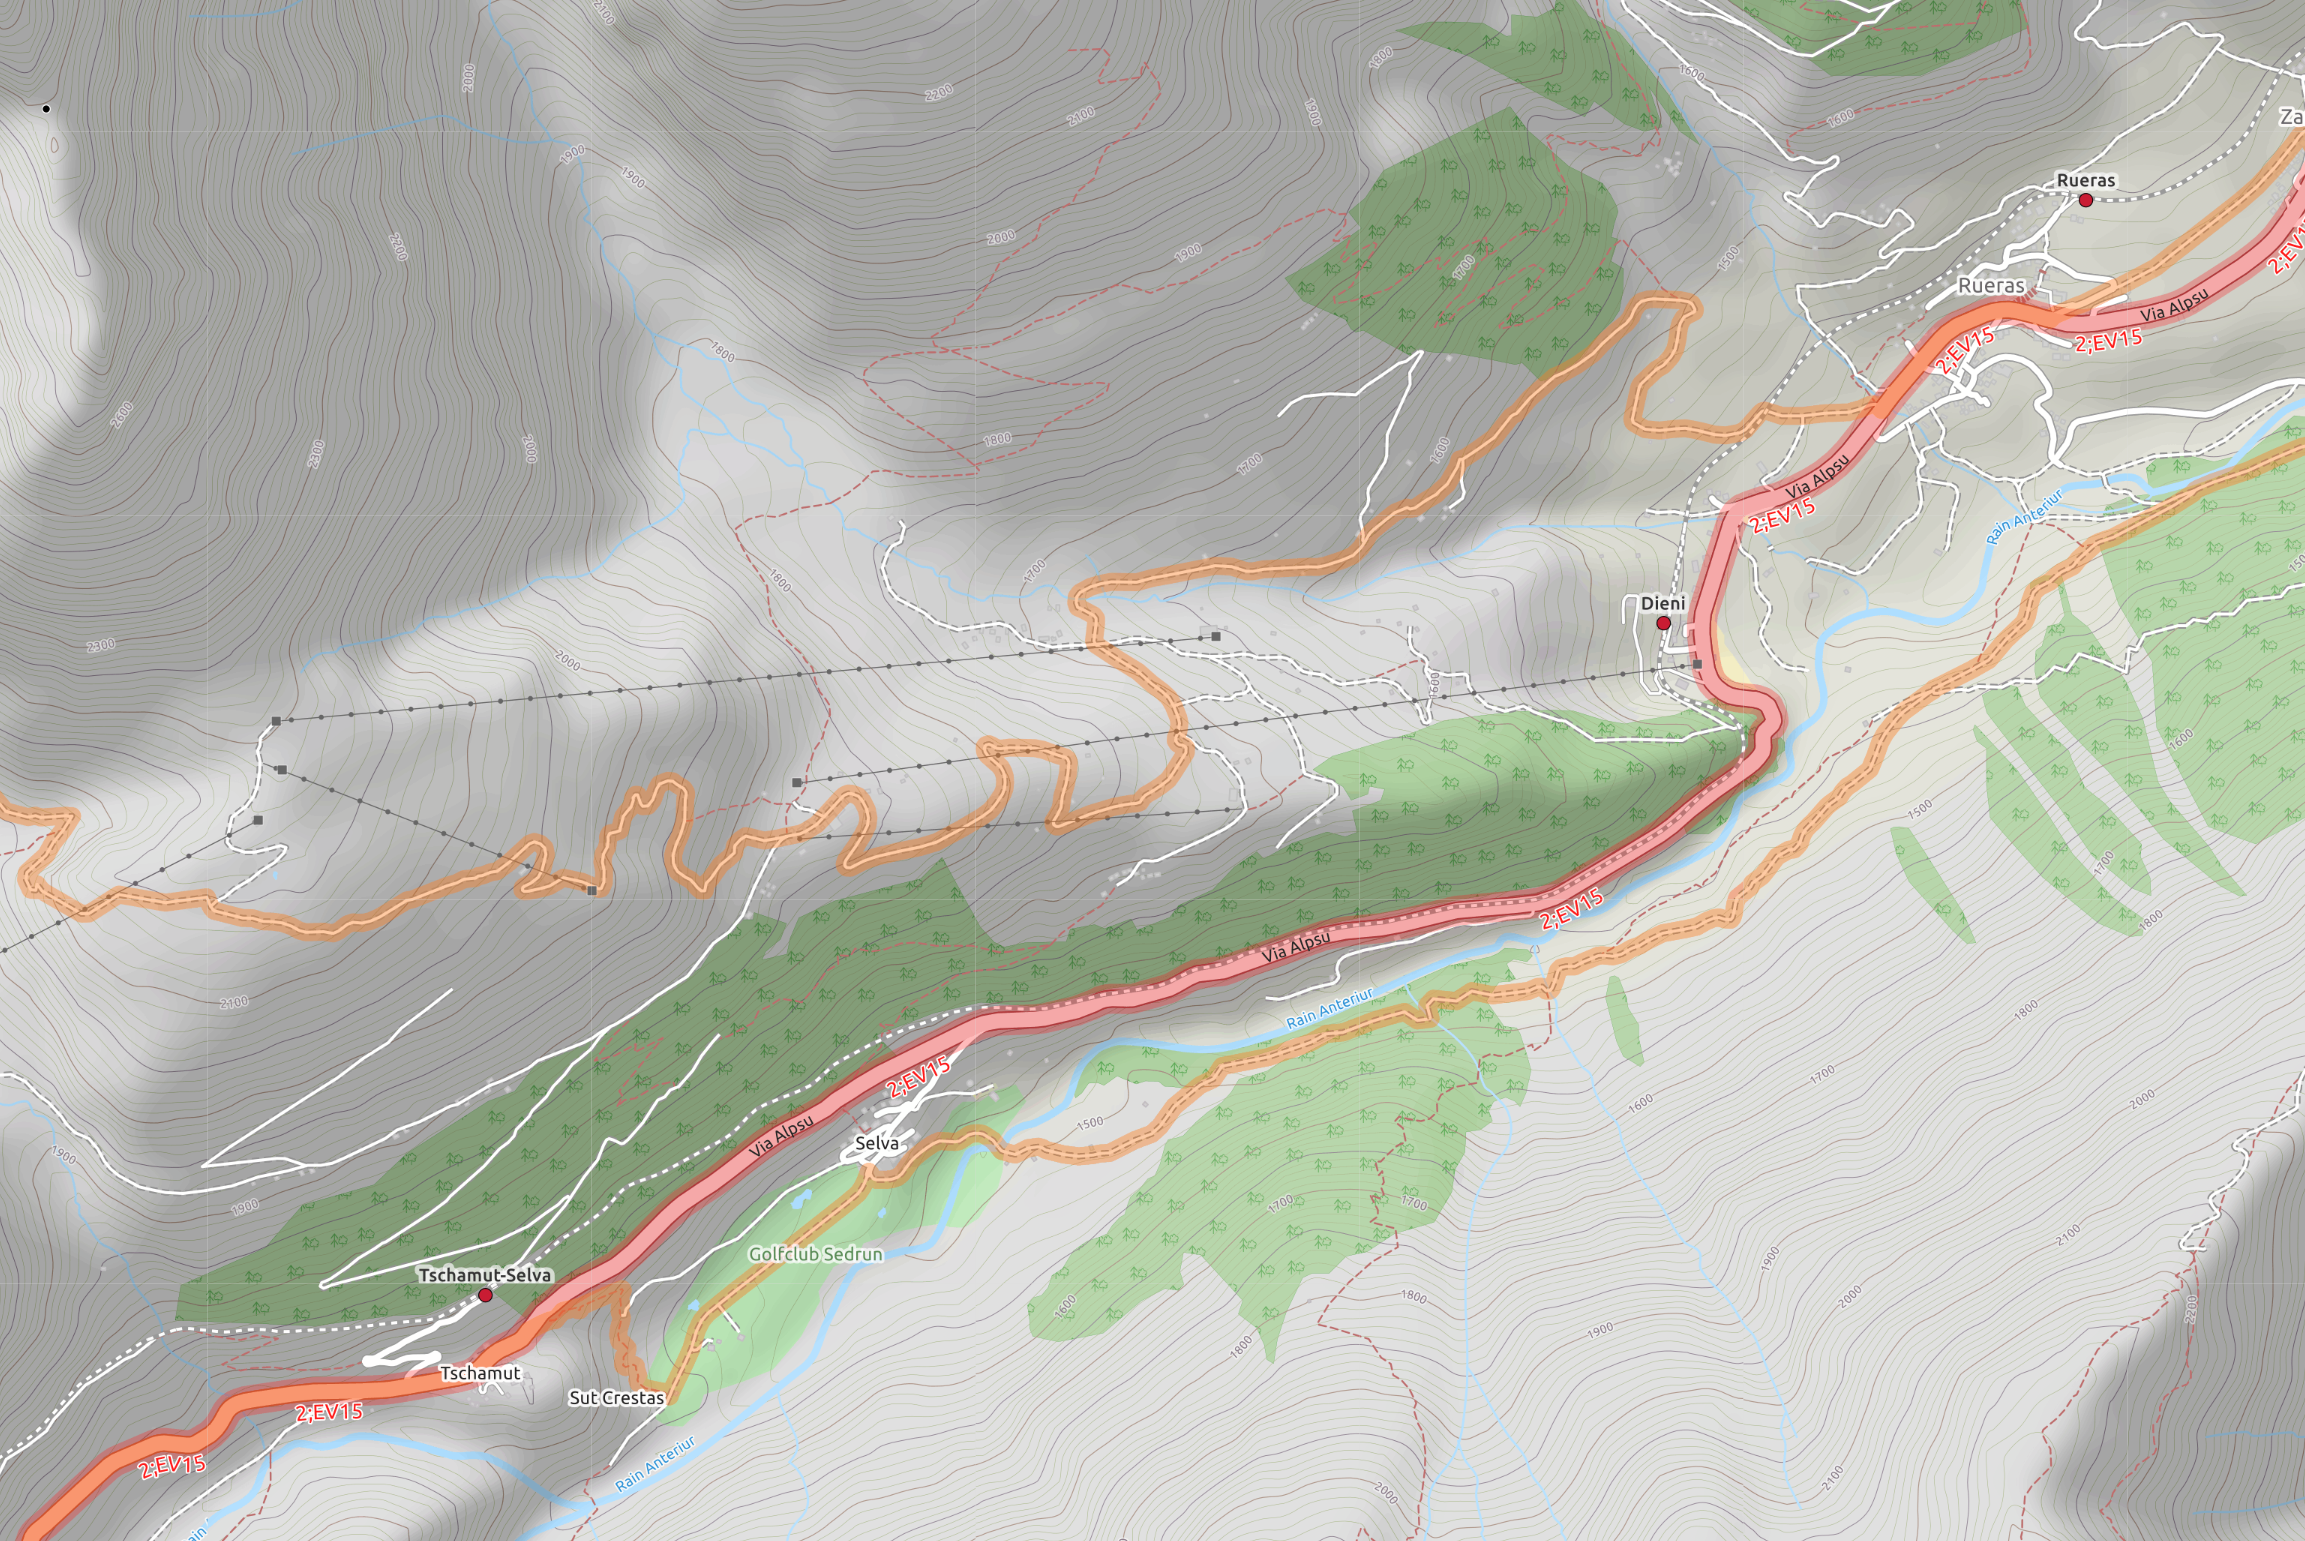
\includegraphics[width=\textwidth]{figures/UppervalleyOSM.png}
	\caption{Upper Valley (Tschamut and Selva) plus Dieni and Rueras from the Lower Valley. Source: Bundesamt für Landestopografie swisstopo.}\footnote{The identical place names in this and in the following figure which are not in boxes refer to train stations.}
	\label{fig:uppervalley}
\end{figure}

\begin{figure}
	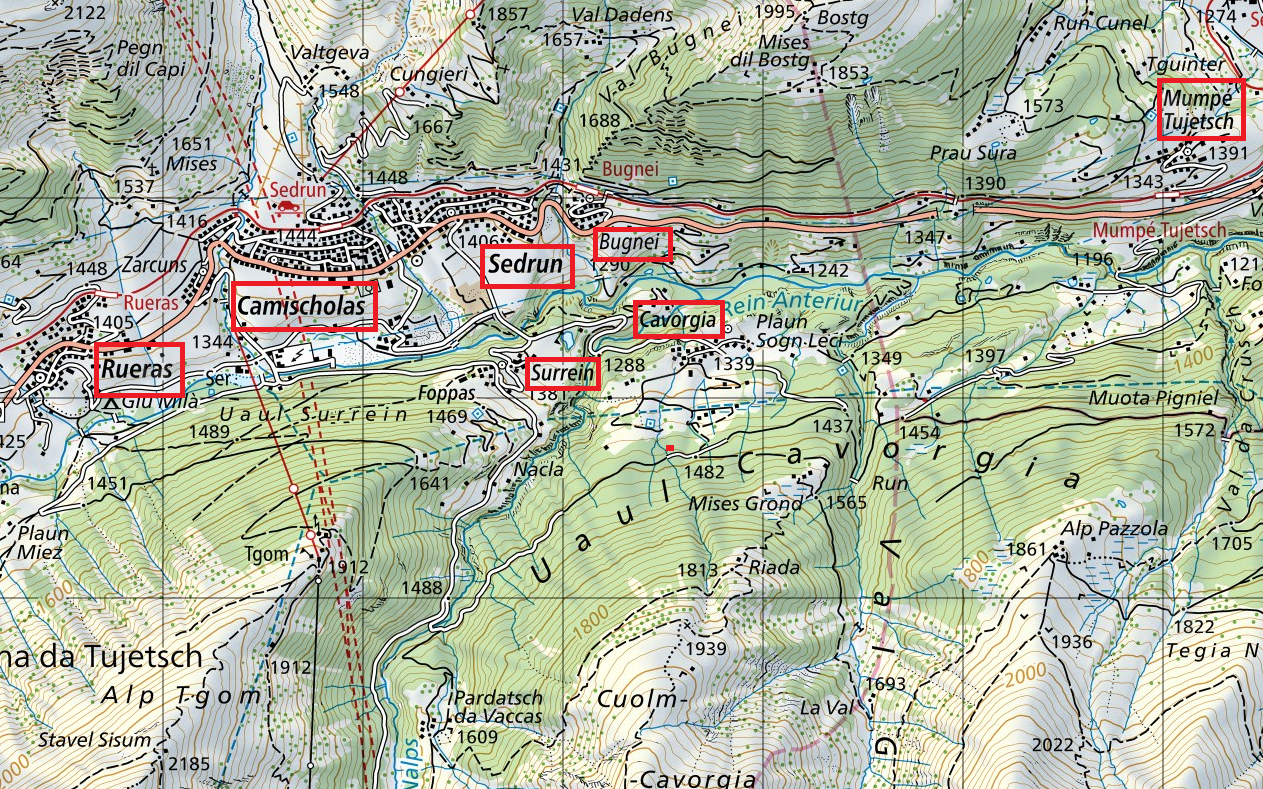
\includegraphics[height=.42\textheight]{figures/Lower Valley fourth.png}
% 	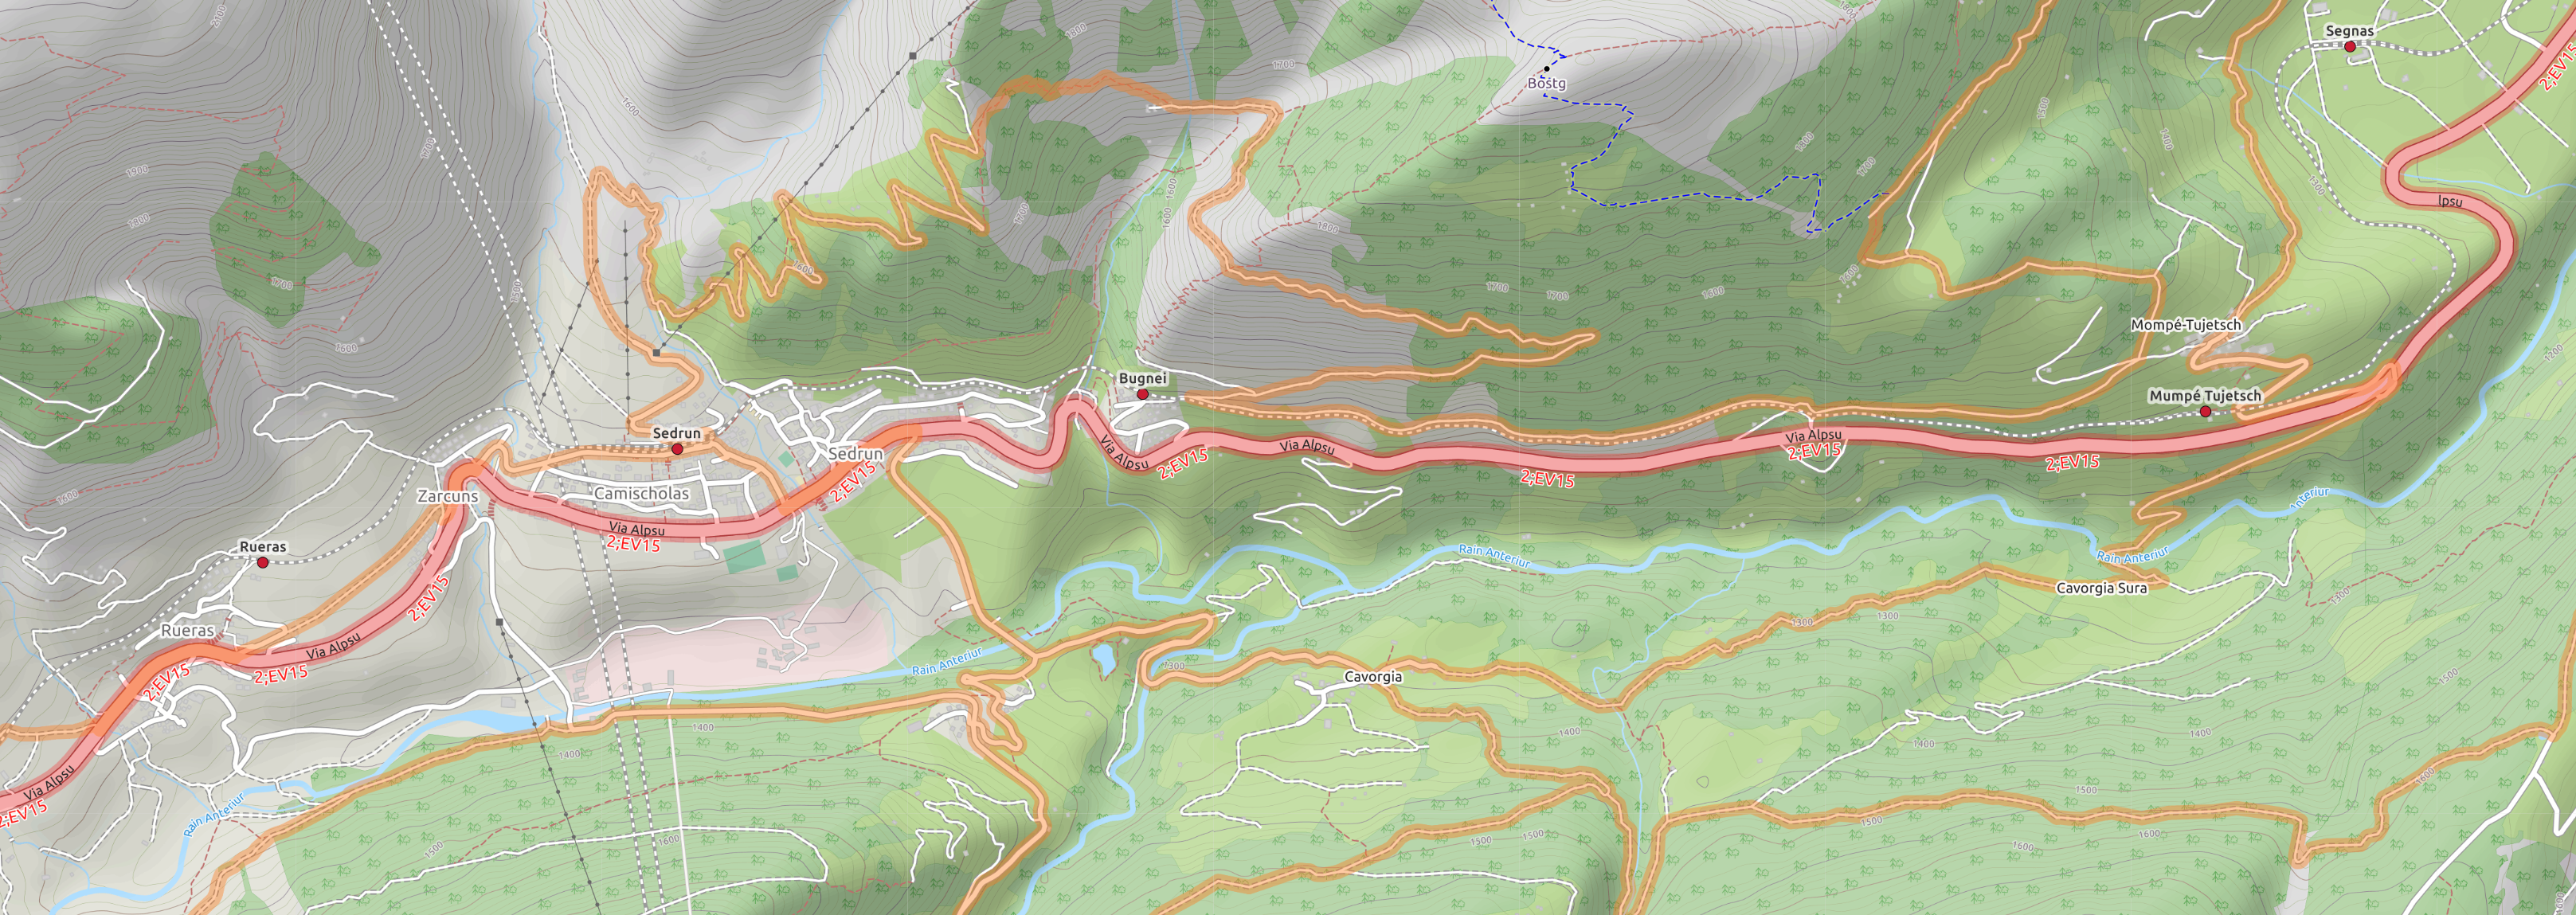
\includegraphics[width=\textwidth]{figures/Lower Valley fourthOSM.png}
	\caption{Lower Valley from Rueras to Bugnei and Mumpé Tujetsch. Source: Bundesamt für Landestopografie swisstopo.}\footnote{In spite of its name, Mumpé Tujétsch is located outside the Tujetsch vally.}
	\label{fig:lowervalley}
\end{figure}

The differences between the two dialects are mostly lexical, whereby the divergent forms of the upper dialect correspond in general to Standard Sursilvan. Some examples are presented in \tabref{difdial} \citep[97]{VicHendry2010}.

\begin{table}
	\caption{Differences between the upper and the lower dialect}
	\label{difdial}
	\begin{tabular}{lllll}
		\lsptoprule
		Lower valley &  Upper valley and Sursilvan & English\\
		\midrule
		\textit{anavaun} & \textit{anavon} & `forward' \\
		\textit{cuntjants} & \textit{cuntents} & `happy' \\
		\textit{sjantar} & \textit{suenter} & `after'\\
		\textit{tgaglja} & \textit{caglia} & `bushes'\\
		\textit{ufaun} & \textit{affon} & `child' \\
		\lspbottomrule
	\end{tabular}
\end{table}

Nowadays there are only very few speakers of the upper dialect left; an example of the variety of Selva is presented in §8.6.

\section{The contact languages of Tuatschin}
The contact languages of Tuatschin are Standard Sursilvan, Swiss German, and Standard German. In this chapter only some few remarks will be given, since the subject is complex and could easily fill a book-length publication. 

Standard Sursilvan is the language of instruction in school and is used among Tuatschin native speakers for written communication.

Contact with Swiss German starts at an early age through contact with Swiss German speakers who have a vacation house in the Tujetsch valley, or with tourists, and also with relatives who live in the German part of Switzerland and who do not understand Romansh.

Standard German starts being taught in school from the fifth form of primary school onwards and is also present through Swiss German and German television. Broadcasts in Romansh are very scarce. Currently there is a ten-minute news broadcast from Monday to Friday, a broadcast for children on Saturday that lasts ten minutes, and a cultural broadcast on Sunday which lasts 25 minutes. Therefore most broadcasts children (and adults) watch are in German.

On a more general level, all Romansh varieties have been in contact with German, Swiss or Standard, for a long time. \citet[176--181]{Liver2010} states that Romansh has been in contact with German since the time of Old High German (ca. 750-1050). Loans from OHG are for instance (I cite the Tuatschin forms) \textit{gljut} `people' (< OHG \textsc{liut}), \textit{uaut} `forest' (< OHG \textsc{wald}), or \textit{lubí} `permit' (< OHG \textsc{laubjan}).

More modern loans are e.g. \textit{ajfach} `simply' (< Swiss German \textit{eifach}), \textit{clétg} `luck' (< German \textit{Glück}), \textit{halt/hald} `simply' (< German \textit{halt}), \textit{ṣchubargjè} `clean' (< Swiss German \textit{suuber mache}), \textit{stédi} `diligent' (< German \textit{stetig}), \textit{schliat/schljats} `bad' (< German \textit{schlecht}). Germanisms which some older native speakers remember but which they do not use any more are \textit{zug} `train', \textit{banhò̱f} `train station' \textit{landstrò̱s} `way', and \textit{hauptstrò̱s} `main way'.

Discourse particles of Swiss German (or Standard German) origin are very often used. Examples are \textit{ábar} `but' (< German \textit{aber}), \textit{álṣò} `this is to say' (< German \textit{also}) \textit{sò} `well, OK' (< German \textit{so}), or \textit{zuar} `though' (< German \textit{zwar}).

Semantic broadening is also frequent. An example is \textit{unfrènda} `sacrifice, casualty', which is derived from Middle Latin \textsc{offerenda} \citep[1283]{Decurtins2012} whose Romance meaning is `sacrifice' and its German one `casualty'.

Calques are also very frequent, especially in the domain of the particle verbs (see §4.1.3). Other examples are \textit{mètar avaun} `imagine' (< German \textit{sich vorstellen}) (note that the Romansh synonym is not reflexive) \textit{curdá sé} (< German auffallen), or \textit{fá cun} `participate' (< German \textit{mitmachen}).

Sursilvan loans are less frequent than Germanisms, which is undoubtedly related to the fact that a huge part of the lexicon Tuatschin shares with Standard Sursilvan has the same form in both varieties.

Examples of sursilvanisms occurring in the corpus are \textit{bugèn} `gladly' instead of \textit{ugèn}, \textit{dumigná} `cope' instead of \textit{dumagnè},  \textit{èl} `in the (\textsc{m})' instead of \textit{ál} or \textit{ájl}, \textit{muossavía} `signpost' instead of \textit{mùssavía}, \textit{Musté} instead of \textit{Mustajr} `Mustér', \textit{ni} `or; right' instead of \textit{né}, \textit{pi} `more' instead of \textit{plé}, \textit{pènṣjunada} `retired (\textsc{f.sg})' instead of \textit{panṣjunada}, \textit{sa} `knows' instead of \textit{sò}, \textit{si} `up' instead of \textit{sé}, \textit{uaul} `forest' instead of \textit{uaut}, \textit{uost} `August' instead of \textit{uést}.

A phonetic influence of Sursilvan is the use of [ʁ] instead of [r], which is not frequent among the native speakers I have consulted, but which one often hears when younger people or children speak Tuatschin.



\section{Glosses}
The glosses used in this grammar are those of the Leipzig Glossing Rules\footnote{https://www.eva.mpg.de/lingua/resources/glossing-rules.php}, to which some glosses have been added.

In order to save space, gender is only indicated on the first element of the noun phrase, excepted in cases where two or more elements of a noun phrase differ in gender. Only plural is indicated since singular is not marked. Indicative mood is not indicated, in contrast to subjunctive, conditional, and imperative mood.

\section{Place names}
In the Romansh examples and texts, I will use the spelling system of this book for the place names. In the English text, I will use the official Sursilvan spelling.

I will not use the German equivalents of the Romansh place names, except if they are used by the consultants themselves.

The place names which occur in this book are presented in \tabref{spellpln}. The German and Italian equivalents are only given for those place names that are located in German- or Italian-speaking areas.

\begin{table}
	\caption{Spelling of place names}
	\label{spellpln}
	\begin{tabular}{lllll}
\lsptoprule
current spelling &  Standard Sursilvan & German/Italian\\
\midrule
\textit{Bugnaj} & \textit{Bugnei}\\
\textit{Camischùlas} & \textit{Camischolas}\\
\textit{Caṣchinùta} & \textit{Caschinutta} & \textit{Göschenen}\\
\textit{Cavòrgja} & \textit{Cavorgia}\\
\textit{Cuéra} & \textit{Cuera} & \textit{Chur}\\
\textit{Diani} & \textit{Dieni}\\
\textit{Dagljégn} & \textit{Dalin}\\
\textit{Gjònda} & \textit{Gonda}\\
\textit{Gljòn} & \textit{Glion}\\
\textit{Lags} & \textit{Laax}\\
\textit{Ligjaun} & \textit{Ligiaun} & \textit{Lugano}\\
\textit{Méjdal} & \textit{Medel}\\
\textit{Nòssadunaun} & \textit{Nossadunnaun} & \textit{Einsiedeln}\\
\textit{Ruèras} & \textit{Rueras}\\
\textit{Sadrún} & \textit{Sedrun}\\
\textit{Ségnas} & \textit{Segnas}\\
\textit{Sèlva} & \textit{Selva}\\
\textit{Surajn} & \textit{Surrein}\\
\textit{Trùn} & \textit{Trun}\\
\textit{Tschamùt} & \textit{Tschamutt}\\
\textit{Turitg} & \textit{Turitg} & \textit{Zürich}\\
\textit{Ursèra} & \textit{Ursera} & \textit{Andermatt}\\
\textit{Zarcúns} & \textit{Zarcuns}\\
\lspbottomrule
\end{tabular}
\end{table}

